\documentclass{report}
\usepackage{amsmath, amssymb}
\usepackage{tikz}
\usetikzlibrary{arrows.meta, positioning, shapes, calc, fit}
\usepackage{geometry}
\usepackage{booktabs}
\usepackage{float}
\usepackage{caption}
\geometry{margin=1in}

\title{Final Project\\MAUI Notes Application\\\large YT0797 C\#.NET Development, Thomas More}
\author{Gilles Van Pellicom}
\date{\today}

\begin{document}
    \maketitle

    \tableofcontents
    \clearpage

% ---------------------------
% Notes
% ---------------------------
    \chapter*{Notes on the Process}
    \addcontentsline{toc}{chapter}{Notes on the Process}

    \section*{Reproducability}
    \begin{itemize}
        \item \textbf{Development and Testing Environment:}
        \begin{itemize}
            \item \textbf{Platform:} macOS Tahoe 26.2
            \item \textbf{Hardware:} M3 Pro, 36\,GB LPDDR5
            \item \textbf{IDE:} Rider 2025.3.0.4
            \item \textbf{Framework:} .NET~9.0.11@arm64, .NET~MAUI 9.0.120/9.0.100
            \item \textbf{Backend Runtime:} ASP.NET 9.0.11
            \item \textbf{Container Platform:} Docker v29.1.2
        \end{itemize}
    \end{itemize}

    All backend components are containerized and can be reproduced using Docker without requiring any local database or API installation. This ensures consistent behavior across development machines and eliminates configuration drift.

% ---------------------------
% Project Overview
% ---------------------------
    \chapter{Project Overview}

    \section{Description}
    This project is a cross-platform notes application built using .NET MAUI. The application targets Android and desktop macOS through Mac Catalyst.

    Users can create, edit, delete, and search textual notes. All note data is persisted in a MySQL database, accessed exclusively through a REST API written in ASP.NET. The MAUI client functions purely as a consumer of this API and does not contain persistence logic.

    \section{High-Level Architecture}
    This project is intentionally split into three layers:

    \begin{itemize}
        \item \textbf{MAUI Client} — Presentation and interaction.
        \item \textbf{ASP.NET REST API} — Application logic and validation.
        \item \textbf{MySQL Database} — Persistent storage.
    \end{itemize}

    Each layer has a clearly defined responsibility. This separation avoids leaking infrastructure concerns into the UI and keeps platform-specific code isolated from business logic.

% ---------------------------
% Requirements
% ---------------------------
    \chapter{Requirements and Fulfillment}

    \section{Functional Requirements}

    \begin{itemize}
        \item \textbf{MVVM architecture:} Implemented using MAUI data binding and view models.
        \item \textbf{CRUD functionality:} Notes can be created, edited, and deleted.
        \item \textbf{Search:} Notes can be queried by matching title and content.
        \item \textbf{Remote persistence:} Notes are stored in a MySQL database.
        \item \textbf{REST-based communication:} All data access occurs via HTTP.
        \item \textbf{Cross-platform support:} Android and macOS (Mac Catalyst).
    \end{itemize}

    \section{Architectural Rationale}
    The decision to introduce an explicit API layer, rather than connecting the MAUI application directly to the database enforces a strict separation of concerns and ensures that persistence logic, validation, and query behavior remain centralized.

    Further, this architecture improves testability. The API can be exercised independently using HTTP tooling, while the MAUI client can be developed and debugged without a direct dependency on database connectivity details. Using MVVM within the client further separates presentation from state management, reducing UI complexity and improving maintainability.

% ---------------------------
% Database Design
% ---------------------------
    \chapter{Database Design}

    \section{Schema}
    The database consists of a single table representing notes.

    \begin{table}[H]
        \centering
        \caption{Notes Table Schema}
        \begin{tabular}{llll}
            \toprule
            \textbf{Column} & \textbf{Type} & \textbf{Attributes} & \textbf{Description} \\
            \midrule
            id      & INT        & PRIMARY KEY, AUTO\_INCREMENT & Unique identifier \\
            title   & LONGTEXT   & NOT NULL & Note title \\
            content & LONGTEXT   & NOT NULL & Note content \\
            date    & TIMESTAMP  & DEFAULT CURRENT\_TIMESTAMP & Creation timestamp \\
            \bottomrule
        \end{tabular}
    \end{table}

    \section{Example Data}

    \begin{table}[H]
        \centering
        \caption{Example Notes}
        \begin{tabular}{p{1cm} p{4cm} p{7cm} p{3cm}}
            \toprule
            $ID$ & $TITLE$ & $CONTENT$ & $DATE$ \\
            \midrule
            1 & MAUI Architecture & Discussion of MVVM bindings, observable properties, command usage, and view model lifecycle behavior in the MAUI client. & 2025-01-10 09:14 \\
            2 & API Design Decisions & Rationale behind REST endpoint structure, stateless request handling, and consistency of JSON payloads. & 2025-01-17 16:02 \\
            3 & Docker Infrastructure & Notes covering Docker Compose orchestration, health checks, volume persistence, and service startup ordering. & 2025-01-24 11:48 \\
            \bottomrule
        \end{tabular}
    \end{table}

% ---------------------------
% Docker
% ---------------------------
    \chapter{Docker Setup}

    \section{Rationale}
    Docker is used to guarantee consistent runtime behavior across development and testing environments. It removes the need for local database setup and ensures that API and database versions remain aligned.

    \section{Docker Compose}
    Docker Compose orchestrates the API and database containers and defines networking, startup order, and persistence behavior.

    Key characteristics of the setup include:

    \begin{itemize}
        \item \textbf{Health checks:} The API only starts once MySQL is fully available.
        \item \textbf{Named volumes:} Database data persists independently of container lifecycle.
        \item \textbf{Service discovery:} Containers communicate using service names rather than hard-coded addresses.
    \end{itemize}

    \section{API Dockerfile}
    The API is built using a multi-stage Dockerfile.

    The build stage compiles and publishes the application using the .NET SDK image. The final stage contains only the published output and the ASP.NET runtime, resulting in a smaller and more secure image. Configuration is supplied through environment variables rather than hard-coded values.

% ---------------------------
% API
% ---------------------------
    \chapter{ASP.NET REST API}

    \section{Overview}
    The API is implemented using ASP.NET and exposes a RESTful interface over HTTP. It is stateless and communicates exclusively via JSON.

    All logic related to validation, ordering, and search behavior resides in the API. The client remains agnostic of storage details and interacts solely through defined endpoints.

    \section{Endpoint Overview}

    \begin{itemize}
        \item \texttt{GET /notes} — Retrieve all notes (newest first)
        \item \texttt{GET /notes/\{id\}} — Retrieve a single note
        \item \texttt{POST /notes} — Create a new note
        \item \texttt{PUT /notes/\{id\}} — Update an existing note
        \item \texttt{DELETE /notes/\{id\}} — Delete a note
        \item \texttt{GET /notes/search?query=...} — Search title and content
    \end{itemize}

    \section{Endpoint Usage}

    \subsection{Retrieval}

    \subsubsection*{Get all notes}
    \begin{verbatim}
curl -X GET "http://localhost:8080/notes"
    \end{verbatim}

    \subsubsection*{Get note by ID}
    \begin{verbatim}
curl -X GET "http://localhost:8080/notes/1"
    \end{verbatim}

    \clearpage
    \subsection{Creation and Modification}

    \subsubsection*{Create a new note}
    \begin{verbatim}
curl -X POST "http://localhost:8080/notes" \
-H "Content-Type: application/json" \
-d '{
  "title": "My Test Note",
  "content": "This is a note created via curl."
}'
    \end{verbatim}

    \subsubsection*{Update an existing note}
    \begin{verbatim}
curl -X PUT "http://localhost:8080/notes/1" \
-H "Content-Type: application/json" \
-d '{
  "title": "Updated title",
  "content": "Updated content",
  "date": "2025-02-01T12:00:00Z"
}'
    \end{verbatim}

    \subsection{Deletion and Search}

    \subsubsection*{Delete a note}
    \begin{verbatim}
curl -X DELETE "http://localhost:8080/notes/1"
    \end{verbatim}

    \subsubsection*{Search notes}
    \begin{verbatim}
curl -X GET "http://localhost:8080/notes/search?query=project"
    \end{verbatim}

% ---------------------------
% Chapter: Application Wiring and MVVM Architecture
% ---------------------------
    \chapter{Application Wiring and MVVM Architecture}

    This chapter describes how this project is wired end-to-end, focusing on the separation of concerns between UI, application logic, transport, and persistence. The MAUI client follows the MVVM pattern strictly, while the backend exposes a narrow REST surface consumed through a dedicated service layer.

    \section{High-Level Architecture}

    This project is composed of two clearly separated applications:

    \begin{itemize}
        \item A \textbf{.NET MAUI client}, responsible for presentation, user interaction, and navigation.
        \item An \textbf{ASP.NET Core REST API}, responsible for persistence, querying, and data integrity.
    \end{itemize}

    The MAUI application never accesses the database directly. All data access is mediated through HTTP calls to the API. This separation keeps the client platform-agnostic and allows the backend to evolve independently.

    \section{MVVM Responsibilities}

    The MAUI application adheres to MVVM without shortcuts or hybrid patterns.

    \subsection{Views}

    Views are implemented as XAML pages and contain no application logic. Their responsibilities are limited to layout and binding.

    \begin{itemize}
        \item UI elements bind to ViewModel properties using MAUI data binding.
        \item User actions (button clicks, item selection) are routed to \texttt{ICommand} instances exposed by the ViewModel.
        \item No services or HTTP clients are referenced from Views.
    \end{itemize}

    \clearpage
    \subsection{ViewModels}

    ViewModels act as the sole owner of UI state and interaction logic.

    \begin{itemize}
        \item Expose observable state using bindable properties and collections.
        \item Translate user intent into service calls.
        \item Perform navigation through MAUI Shell routing.
    \end{itemize}

    ViewModels are unaware of transport details such as URLs, JSON, or HTTP verbs. Their dependency is expressed only in terms of interfaces.

    \subsection{Service Layer}

    The service layer provides a thin abstraction over the REST API.

    \begin{itemize}
        \item \texttt{INotesApiService} defines the contract for note operations.
        \item \texttt{NotesApiService} implements this contract using \texttt{HttpClient}.
        \item Serialization and endpoint mapping are contained entirely within this layer.
    \end{itemize}

    This indirection prevents HTTP concerns from leaking into ViewModels and keeps the application testable.

    \section{Dependency Injection and Composition}

    All wiring is performed in \texttt{MauiProgram.cs}, which acts as the composition root.

    \begin{itemize}
        \item ViewModels and Views are registered with appropriate lifetimes.
        \item A platform-aware \texttt{HttpClient} is configured once and reused.
        \item Services are injected via constructors, not resolved manually.
    \end{itemize}

    This ensures a single, explicit location where object lifetimes and dependencies are defined.

    \section{Backend Wiring Overview}

    On the backend side, the ASP.NET API follows a similarly layered approach.

    \begin{itemize}
        \item Controllers expose REST endpoints only.
        \item Entity Framework Core handles database access via \texttt{NotesDbContext}.
        \item The controller depends on the DbContext through dependency injection.
    \end{itemize}

    No business logic is embedded in the controller beyond basic validation and request handling. Persistence logic remains confined to the data layer.

    \section{End-to-End Interaction Flow}

    The following diagram illustrates the complete interaction path, from user action to persistence and back. Each layer communicates only with its immediate neighbor.

    \begin{figure}[H]
        \centering
        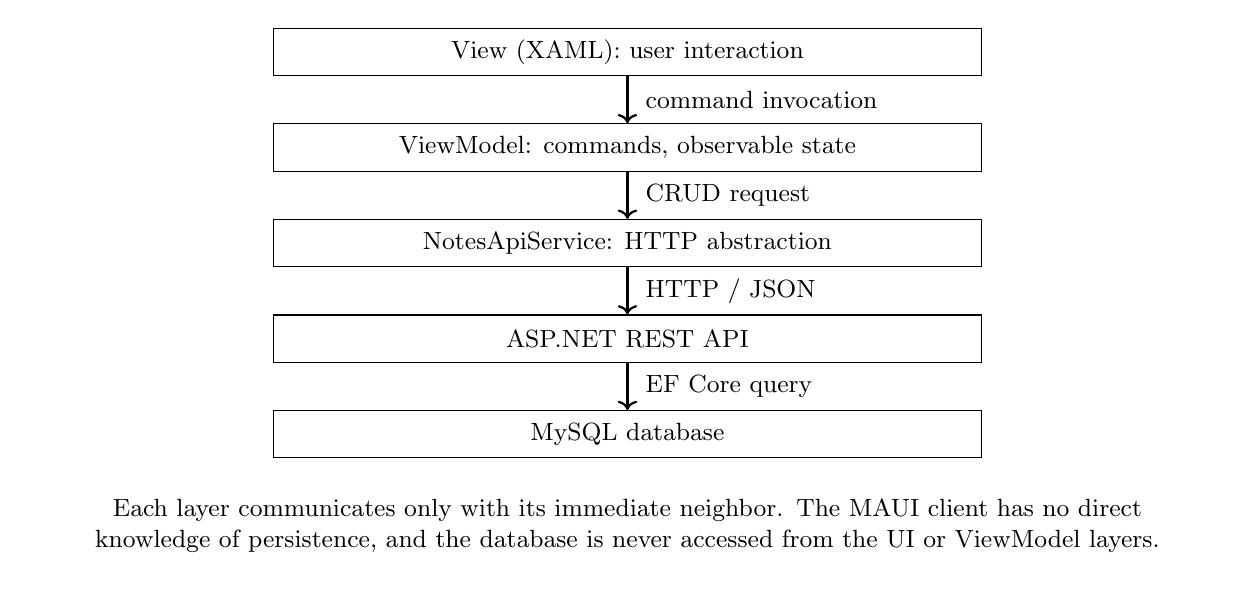
\begin{tikzpicture}[node distance=6mm, every node/.style={font=\small}]
            % blocks
            \node (view) [draw, rectangle, minimum width=9cm, minimum height=6mm]
            {View (XAML): user interaction};

            \node (vm) [draw, rectangle, below=of view, minimum width=9cm, minimum height=6mm]
            {ViewModel: commands, observable state};

            \node (service) [draw, rectangle, below=of vm, minimum width=9cm, minimum height=6mm]
            {NotesApiService: HTTP abstraction};

            \node (api) [draw, rectangle, below=of service, minimum width=9cm, minimum height=6mm]
            {ASP.NET REST API};

            \node (db) [draw, rectangle, below=of api, minimum width=9cm, minimum height=6mm]
            {MySQL database};

            % arrows
            \draw[->, thick] (view.south) -- (vm.north)
            node[midway, right, xshift=1mm] {command invocation};

            \draw[->, thick] (vm.south) -- (service.north)
            node[midway, right, xshift=1mm] {CRUD request};

            \draw[->, thick] (service.south) -- (api.north)
            node[midway, right, xshift=1mm] {HTTP / JSON};

            \draw[->, thick] (api.south) -- (db.north)
            node[midway, right, xshift=1mm] {EF Core query};

            % note
            \node (note) [below=of db, align=center, text width=15cm, yshift=2mm]
            {Each layer communicates only with its immediate neighbor. The MAUI client has no direct knowledge of persistence, and the database is never accessed from the UI or ViewModel layers.};

        \end{tikzpicture}
        \caption{End-to-end user interaction and data flow across the MAUI client and backend API.}
    \end{figure}

    \section{Architectural Rationale}

    This wiring enforces clear boundaries:

    \begin{itemize}
        \item UI changes do not affect persistence or transport logic.
        \item API changes are localized to the service layer.
        \item Platform-specific concerns remain outside application logic.
    \end{itemize}

    The result is a codebase that is predictable to reason about, straightforward to extend, and resistant to architectural drift as the project grows.

% ---------------------------
% Platform Integration
% ---------------------------
    \chapter{Platform-Specific Configuration}

    \section{Android}
    The Android manifest defines permissions and application-level configuration.

    \begin{verbatim}
<?xml version="1.0" encoding="utf-8"?>
<manifest xmlns:android="http://schemas.android.com/apk/res/android"
          package="com.finalproject.maui_app">

    <uses-permission android:name="android.permission.ACCESS_NETWORK_STATE"/>
    <uses-permission android:name="android.permission.INTERNET"/>

    <application android:networkSecurityConfig="@xml/network_security_config"
                 android:enableOnBackInvokedCallback="true"></application>
</manifest>
    \end{verbatim}

    One detail which might feel unfamiliar to native Android developers is that the \texttt{application} tag is intentionally empty. In .NET MAUI, application wiring and lifecycle integration are generated at build time unless explicitly overridden. The manifest therefore acts as a declarative configuration layer rather than a full application definition.

    \section{macOS (Mac Catalyst)}
    macOS applications require explicit entry points and lifecycle integration.

    \begin{itemize}
        \item \textbf{Info.plist:} Declares application capabilities, including network access and background behavior.
        \item \textbf{AppDelegate.cs:} Integrates with the native macOS application lifecycle and handles OS-level events.
        \item \textbf{Program.cs:} Defines the application entry point and initializes the MAUI host for Mac Catalyst.
    \end{itemize}

    These files provide the necessary bridge between MAUI’s cross-platform abstractions and macOS’ native application model, which remains more explicit than its mobile counterparts.

% ---------------------------
% Outcome
% ---------------------------
    \chapter{Outcome}

    This project resulted in a functional cross-platform notes application with a clear separation between presentation, application logic, and persistence.

    Both Android and macOS builds were tested successfully. The backend infrastructure is fully reproducible using Docker, and the architecture allows future extensions without structural changes to existing components. A video recording of a demonstration of this project will be provided seperately.

\end{document}